\chapter{Preliminares}
\label{chap:introduction}

La música constituye una parte fundamental de la sociedad humana. Desde una perspectiva antropológica, puede considerarse como uno de los elementos fundacionales de múltiples culturas, al igual que las matemáticas. Ambas disciplinas comparten un impulso común: encontrar regularidad dentro de la complejidad. A partir de una motivación personal, en este trabajo se desarrollarán herramientas teóricas y marcos conceptuales que permitan explorar la intersección entre estas dos disciplinas.

El objetivo de este trabajo es caracterizar piezas musicales de manera matemática y utilizar herramientas computacionales para obtener un análisis congruente. En particular, se busca modelar la evolución melódica como un proceso estocástico en tiempo discreto y, posteriormente, incorporar estructura subyacente no directamente observable. Para ello se empleará la teoría de cadenas de Markov y, en especial, una subrama conocida como cadenas de Markov ocultas, las cuales permiten modelar sistemas dinámicos estocásticos con estados no observables directamente.

Una pieza musical puede entenderse, en primera aproximación, como una organización de eventos sonoros en el tiempo. Para convertir esa intuición en una formulación matemática se necesita fijar, al menos, tres componentes: (i) qué aspectos del sonido se consideran como información relevante, (ii) cómo se discretiza el tiempo musical, y (iii) qué tipo de dependencia se permitirá entre eventos consecutivos.

Desde un punto de vista musical, los eventos sonoros suelen describirse mediante altura (nota), duración (ritmo) y su relación con otros eventos simultáneos o consecutivos (armonía y melodía). En esta tesis se privilegia el componente melódico como objeto principal de observación: una melodía es una sucesión ordenada de notas en el tiempo. Esta elección no es meramente estética; es la que permite articular con claridad el puente hacia procesos estocásticos discretos.

El objetivo de esta parte no es desarrollar teoría musical exhaustiva, sino fijar una base mínima que justifique la representación matemática adoptada y clarifique qué se pierde y qué se conserva con las simplificaciones del modelo.

\textit{Altura (notas y clases de altura).} En el sistema occidental, las alturas musicales se organizan de manera discreta. En un instrumento como el piano, esta discretización se observa físicamente: el teclado presenta un conjunto finito de teclas por octava, y cada tecla corresponde a una frecuencia bien definida. Esta estructura permite modelar las notas como símbolos pertenecientes a un alfabeto finito. Dependiendo del nivel de abstracción, es común distinguir entre (a) \emph{notas con registro} (por ejemplo, $C_4, D_4, \dots$) y (b) \emph{clases de altura} (por ejemplo, $C, D, \dots$ identificadas módulo octava). En este trabajo se adopta un conjunto finito $S$ de símbolos musicales cuyo contenido depende de la pieza y de la representación elegida; dicho conjunto constituye el espacio de estados del modelo.

Una representación visual estándar de este conjunto discreto de alturas es el teclado del piano, en el cual las notas se disponen de manera lineal y ordenada, sugiriendo de forma natural una estructura de estados sobre la cual se definen transiciones probabilísticas.

\begin{figure}[h]
\centering
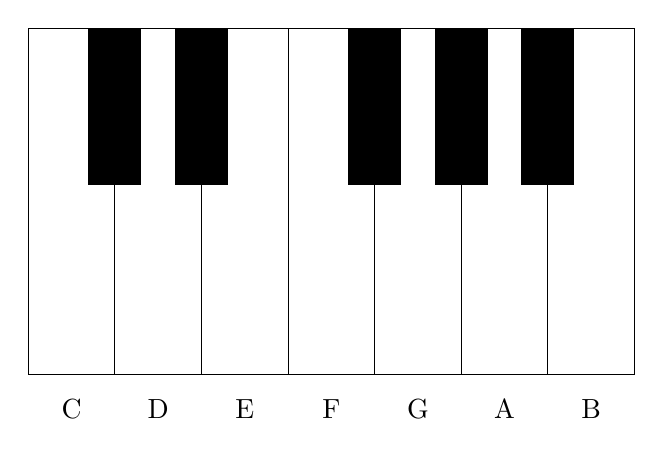
\begin{tikzpicture}[scale=1.1]

% Teclas blancas
\draw[fill=white] (0,0) rectangle (1,4);
\draw[fill=white] (1,0) rectangle (2,4);
\draw[fill=white] (2,0) rectangle (3,4);
\draw[fill=white] (3,0) rectangle (4,4);
\draw[fill=white] (4,0) rectangle (5,4);
\draw[fill=white] (5,0) rectangle (6,4);
\draw[fill=white] (6,0) rectangle (7,4);

% Teclas negras
\draw[fill=black] (0.7,2.2) rectangle (1.3,4);
\draw[fill=black] (1.7,2.2) rectangle (2.3,4);
\draw[fill=black] (3.7,2.2) rectangle (4.3,4);
\draw[fill=black] (4.7,2.2) rectangle (5.3,4);
\draw[fill=black] (5.7,2.2) rectangle (6.3,4);

% Etiquetas
\node at (0.5,-0.4) {C};
\node at (1.5,-0.4) {D};
\node at (2.5,-0.4) {E};
\node at (3.5,-0.4) {F};
\node at (4.5,-0.4) {G};
\node at (5.5,-0.4) {A};
\node at (6.5,-0.4) {B};

\end{tikzpicture}
\caption{Representación esquemática de una octava en el teclado del piano.}
\end{figure}

\textit{Ritmo y discretización temporal.} El ritmo establece la estructura temporal de la música y determina cuándo ocurren los eventos. Desde el punto de vista matemático, esto sugiere indexar la melodía mediante un parámetro temporal discreto $n\in\mathbb{N}$. En esta tesis se adopta una simplificación deliberada: se considera una malla temporal uniforme. Bajo este supuesto, cada instante de tiempo corresponde a una posición en la secuencia y el proceso musical puede representarse como una sucesión indexada $\{X_n\}_{n\ge 0}$ donde $X_n$ describe la información musical relevante en el instante $n$. Este paso implica una decisión de modelado: fenómenos como síncopas, rubato o cambios de tempo quedan fuera de la representación si no se incorporan explícitamente mediante un refinamiento temporal o variables adicionales. Aun así, la discretización uniforme constituye un punto de partida natural para el análisis computacional de melodías en notación simbólica.

\textit{Melodía, continuidad y dependencia local.} Musicalmente, una melodía no es una colección aleatoria de notas: exhibe continuidad y regularidades locales. Por ejemplo, después de una nota dada suele haber preferencia por movimientos conjuntos (intervalos pequeños) frente a saltos grandes, o bien aparecen patrones típicos (motivos) que tienden a repetirse con variaciones. Estas regularidades sugieren dependencia estocástica entre eventos consecutivos.

\textit{Armonía como estructura subyacente.} La armonía introduce relaciones simultáneas entre notas y define una organización implícita de acordes y funciones tonales. Crucialmente, dicha organización no siempre es directamente observable a partir de una sola línea melódica: una melodía puede ser compatible con varias interpretaciones armónicas, y aun así la armonía influye en qué notas son más probables en cada momento. Esta separación entre lo que se observa (notas melódicas) y lo que condiciona (contexto armónico) anticipa el paso hacia variables latentes y, por tanto, hacia cadenas de Markov ocultas.

Con estos elementos, una melodía queda representada como una sucesión de variables aleatorias
\[
(X_n)_{n\ge 0}, \qquad X_n\in S,
\]
donde $S$ es finito y corresponde a las alturas (o clases de altura) admitidas por la representación.

Una primera suposición extrema sería asumir independencia entre $X_0,X_1,\dots$, pero esto es difícil de justificar musicalmente: la elección de una nota suele depender del contexto inmediato. En el otro extremo, permitir que $X_{n+1}$ dependa de todo el historial produce un modelo muy costoso de estimar a partir de una sola pieza o de un corpus reducido. En consecuencia, emerge una hipótesis intermedia que es a la vez musicalmente interpretable y matemáticamente manejable: que el futuro dependa solamente del presente. Esta hipótesis es precisamente la propiedad markoviana.

\begin{Definicion}
Sea $(\Omega,\mathcal{F},\mathbb{P})$ un espacio de probabilidad. Una sucesión de variables aleatorias $\{X_n\}_{n \geq 0}$ con valores en un conjunto de estados $S$ se denomina \emph{cadena de Markov} si, para todo $n \geq 0$ y para cualesquiera $i_0, \ldots, i_n, j \in S$, se cumple
\[
P(X_{n+1} = j \mid X_n = i_n, \ldots, X_0 = i_0)
=
P(X_{n+1} = j \mid X_n = i_n).
\]
En forma abreviada, esta propiedad suele expresarse como
\[
P(X_{n+1}=i_{n+1}\mid X_n=i_n,\dots,X_0=i_0)=P(X_{n+1}=i_{n+1}\mid X_n=i_n).
\]
\end{Definicion}
\
En el contexto musical, el supuesto markoviano afirma que la probabilidad de la próxima nota depende únicamente de la nota actual. Esta simplificación no pretende capturar toda la gramática musical; su papel es aislar y cuantificar dependencias locales que, en muchos estilos, explican una parte relevante de la coherencia melódica.

Si el proceso se encuentra en el estado $i$, se supone que la probabilidad de transitar al estado $j$ es constante y se denota por $P_{ij}$:
\[
P(X_{n+1}=j\mid X_n=i)=P_{ij}.
\]
Estas probabilidades satisfacen
\[
P_{ij}\ge 0,\qquad \sum_{j\in S}P_{ij}=1.
\]
La matriz $\mathbf{P}=(P_{ij})_{i,j\in S}$ se denomina \emph{matriz de transición} \cite{ross2014} y encapsula la dinámica del modelo:
\[
\mathbf{P}=
    \begin{Vmatrix}
       P_{00} & P_{01} & P_{02} & \ldots \\
       P_{10} & P_{11} & P_{12} & \ldots\\
       \vdots & \vdots & \vdots & \ldots \\
       P_{i0} & P_{i1} & P_{i2} & \ldots\\
       \vdots & \vdots & \vdots & \ldots \\
    \end{Vmatrix}.
\]

En aplicaciones musicales, la matriz de transición no se especifica de manera teórica, sino que se estima empíricamente a partir de la partitura. Para cada estado $i\in S$ se contabiliza el número de veces que la nota correspondiente es seguida por cada nota $j\in S$, y se normaliza por el número total de ocurrencias de $i$. Así se obtiene un estimador de máxima verosimilitud de las probabilidades de transición, garantizando que cada renglón de $\mathbf{P}$ define una distribución de probabilidad.

Este procedimiento induce una cadena de Markov homogénea cuya estructura refleja regularidades locales de la melodía. En particular, la dependencia entre notas consecutivas queda codificada en $\mathbf{P}$, mientras que el espacio de estados captura el registro y el vocabulario melódico efectivo de la pieza. La motivación intrínseca de este modelo es caracterizar una melodía para, por un lado, entenderla con mayor profundidad y, por otro, replicarla o generar secuencias compatibles con su estilo, en el sentido estadístico local que impone la matriz de transición.
\begin{Definicion}
Un vector de probabilidad $\boldsymbol{\pi}$ se denomina \emph{distribución estacionaria} si satisface
\[
\boldsymbol{\pi}=\boldsymbol{\pi}\mathbf{P}.
\]
Si la cadena es irreducible y aperiódica, existe una única distribución estacionaria y se cumple que
\[
\lim_{n\to\infty}P(X_n=j\mid X_0=i)=\pi_j.
\]

\end{Definicion}


En el contexto musical, la distribución estacionaria describe el comportamiento estadístico global del modelo y puede interpretarse como la frecuencia relativa de aparición de cada nota en el largo plazo. En otras palabras, mientras $\mathbf{P}$ captura las dependencias locales (qué suele seguir a qué), $\boldsymbol{\pi}$ ofrece una descripción agregada del peso de cada nota dentro de la melodía, lo cual resulta útil para comparar estilos o identificar centros de gravedad melódicos.



Hasta aquí se ha considerado que la melodía observada coincide con el estado del proceso, es decir, que $X_n$ es directamente observable. Esta hipótesis es adecuada como primer modelo, pero sugiere una limitación importante: muchas regularidades musicales no se explican únicamente por la nota anterior, sino por un contexto estructural más profundo.

En particular, la armonía actúa como una organización subyacente que condiciona cuáles notas son plausibles en cada instante. Aunque una melodía sea observable, el contexto armónico que la gobierna puede no serlo de manera directa y unívoca. Desde una perspectiva probabilística, esto sugiere la existencia de variables latentes que evolucionan en el tiempo y que influyen en la distribución de las observaciones. Dicho de otra forma, la melodía puede verse como la salida observable de un sistema dinámico estocástico cuya dinámica interna no se observa completamente.

Esto conduce al problema que dará paso al siguiente capítulo: \emph{modelar la melodía como un proceso estocástico en el que la estructura armónica subyacente se representa mediante estados ocultos}. La hipótesis markoviana es razonable en este nivel latente porque las progresiones armónicas suelen exhibir dependencia local (por ejemplo, ciertas funciones tienden a seguir a otras), mientras que las notas observadas pueden interpretarse como emisiones condicionadas por dicho estado armónico. La formalización matemática de esta idea conduce a las \emph{cadenas de Markov ocultas}, que constituyen el marco principal de esta tesis y se desarrollarán a continuación.
